\section{Datenbus}
Eines der Hauptbestandteile des modularen Eingabesystems ist das Entwerfen und Umsetzen eines leistungsfähigen und flexiblen Datenbusses. Dieser Datenbus dient als Kommunikationsschnittstelle zwischen den verschiedenen Modulen, wie dem Keypad-Modul und dem Audiomodul und ermöglicht dadurch die Datenübertragung zum Hauptmodul. Skalierbarkeit, Zuverlässigkeit und Geschwindigkeit sind die Hauptkriterien des Datenbusses. Ziel ist es, eine einfache Erweiterbarkeit durch Hinzufügen oder Entfernen von Modulen zu ermöglichen, ohne dabei grundlegende Kommunikationsmechanismen zu beeinträchtigen.

\section{Aufbau des Datenbusses}
Der Bus ist nach folgendem Schema aufgebaut:
\begin{itemize}
    \item Start of Frame (SOF) - 2 Bit zum Synchronisieren der Frequenzen
    \item Sendeadresse -  3 Bit zum Senden der Adresse
    \item Content of Frame (COF) - 3 Bit für Datenlänge in Byte
    \item Daten - X Byte
    \item ?? (CRC) - X Bit
    \item Enf of Frame (EOF) - 4 Bit LOW, Signalende
\end{itemize}

Die folgende Abbildung stellt den Datenbus dar:
\begin{figure}[H]
    \centering    
    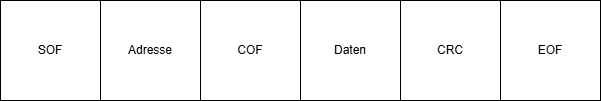
\includegraphics[width=1\textwidth]{Bilder/datenbus.png}
    \caption{Aufbau des Datenbusses}
    \label{Datenbus}
\end{figure}
